%************VERSUCHSANORDNUNG*************
\section{Experimental Setup}
\label{sec:versuchsandordnung}
The experimental work done in this thesis primarily utilized a Low-Temperature Scanning Tunneling Microscope setup (LT-STM).
This STM is composed of two distinct compartments, the preparation chamber (PC) the measurement chamber (MC).
The sample is inserted through a airlock into the preparation chamber.
In the whole system there is in a Ultra High Vacuum (UHV) at about 10$^{-11}$ - 10$^{-10}$ mbar, which is archieved by four individuall pumps.
The base Vacuum is achieved with the turbomolecular pump and the scroll pump through the airlock.
Additionally there is a titanium sublimation pump and a ion pump in the preparation room.

\monofig{width=\textwidth}{Experimental_Setup/STM_Picture_1_edited.pdf}{
    The experimental setup used, 
    A: cooling-chamber filled with Liquid Oxigen,
    B: measuring-chamber with spring suspended sample holder and tip,
    C: sputter-gun,
    D: metal-evaporater,
    E: molecule-evaporater,
    F: preparation-chamber with free movable sample holder arm,
    G: LEED system,
    H: Electronic used to monitor the function of the STM}{fig:stm_uni_kf}
%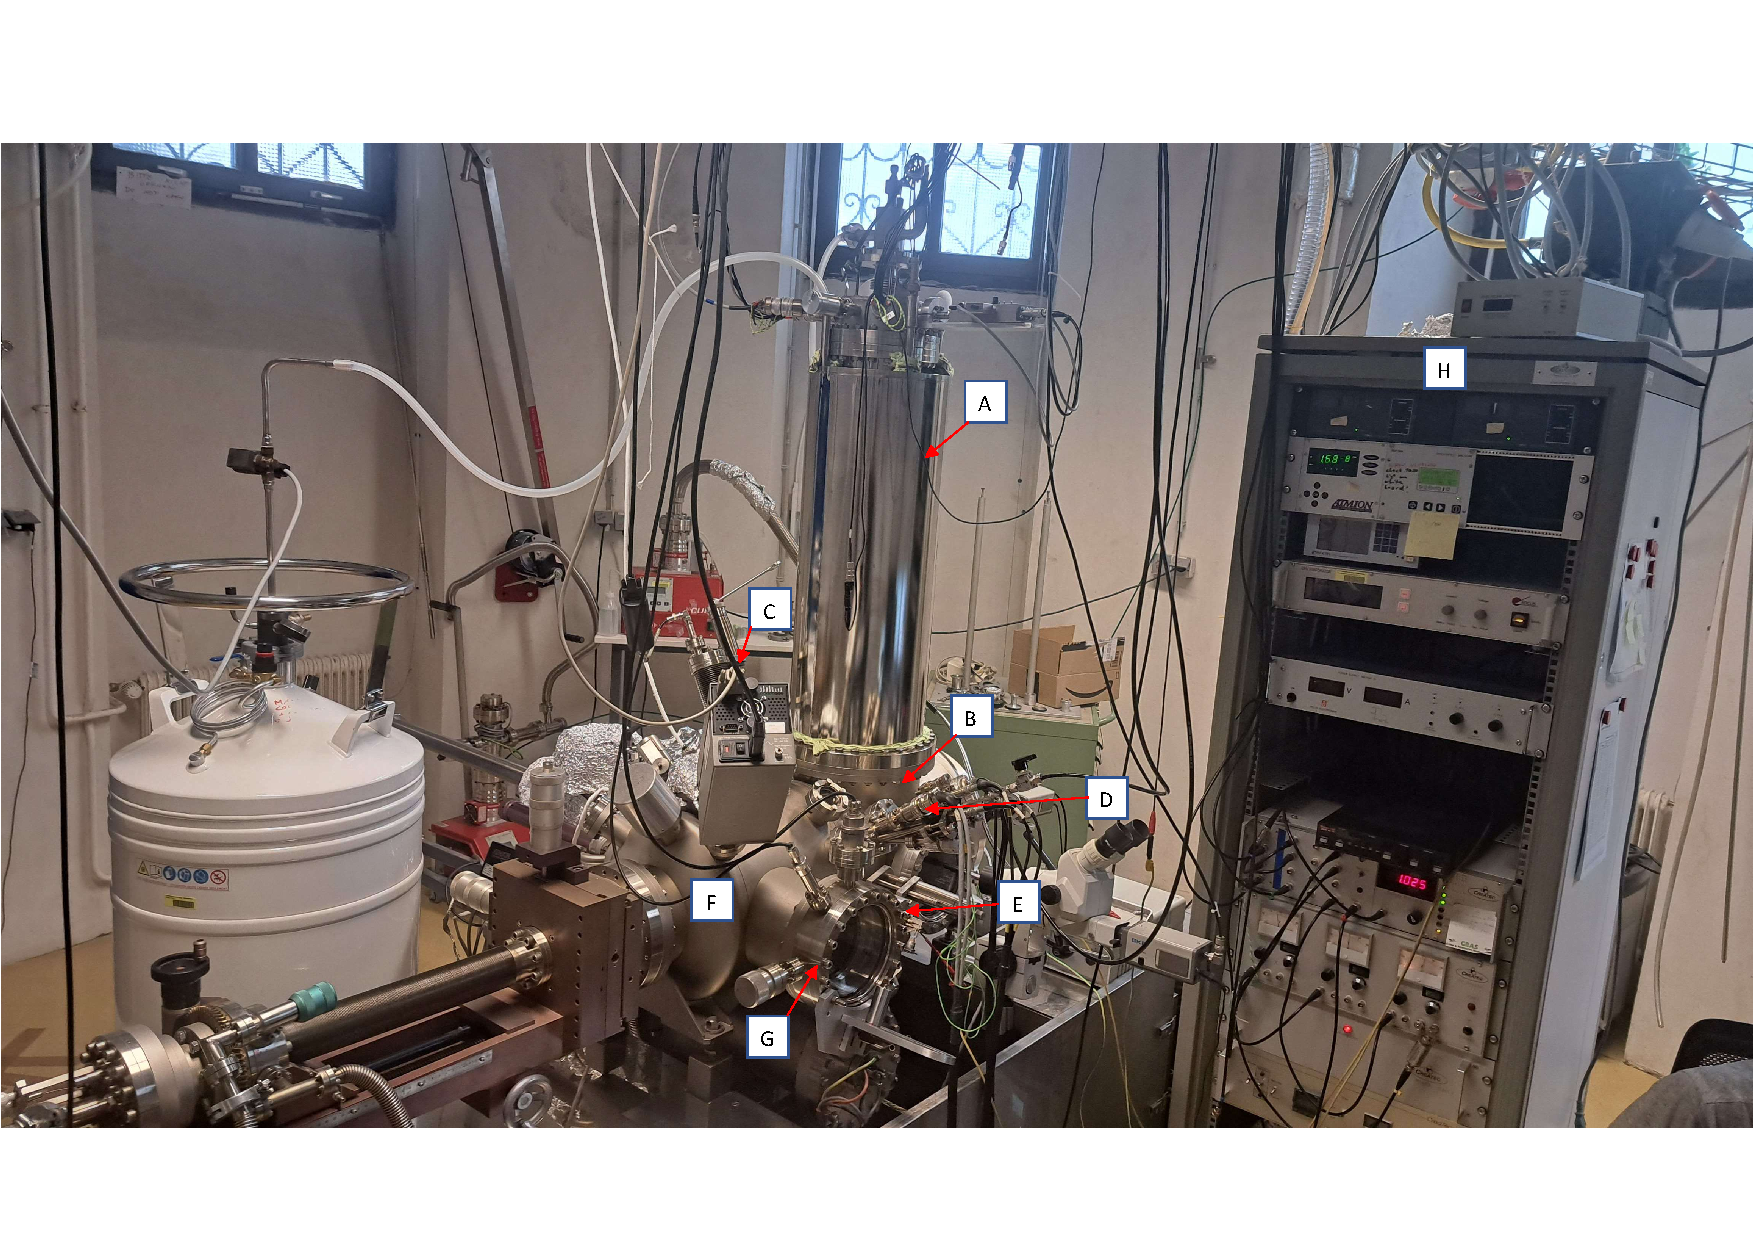
\includegraphics[width=0.9\textwidth]{Experimental_Setup/STM_Picture_1_edited.pdf}

The Probe-holder can be moved in each direction and rotated using an integrated arm in the PC.
It is also used to insert the Probe-holder into the MC.
The PC is equipped with a LEED system, which fluorescent screen can be extended. 
Additionally the PC has a metal-evaporator and organic-molecule evaporator (e-beam evaporator with a triple Knudsen cell) which are used to deposit submono- or monolayer structres onto an circular sample (10 mm x 2 mm).
This sample is mounted onto the previously mentioned Probe-holder, a Heatwaves Labs Inc. button heater with a resistive heating range of 20 K - 900 K.
The sample can also be cooled using LN2 or LHe through built-in pipe system in the manipulator arm.
A Quartz-Crystal Microbalance (QCM) with sub Angstöm precision is used to monitor the deposition thickness.
To clean the sample, an Argon sputter gun is employed, which utilizes an electric field to ionize and accelerate the argon gas.
The MC consists of a LT-STM which is surrounded by a two-shell cryostat, to which it is fixed, and two radiation shields to archieve temperatures as low as 7 K.
In this thesis the cryostat chamber was filled with LN2 which means it was oparated at 75 K.
The primary measuring unit (tip and sample storage place) is vibrationally damped using a coupled spring system.